\chapter{Revogação de Assinaturas PGP}

\section{Localização de um Certificado para Assinar}
Primeiramente, foi necessário localizar um certificado PGP de outra pessoa para assinar \cite{gnupgkeysigning}:

\begin{lstlisting}[language=bash]
# Busca por certificados PGP que o Enzo Nicolas publicou no forum da disciplina
gpg --keyserver keyserver.ubuntu.com --recv-keys 24B83FFEA53408DA
\end{lstlisting}

\begin{figure}[htb]
    \centering
    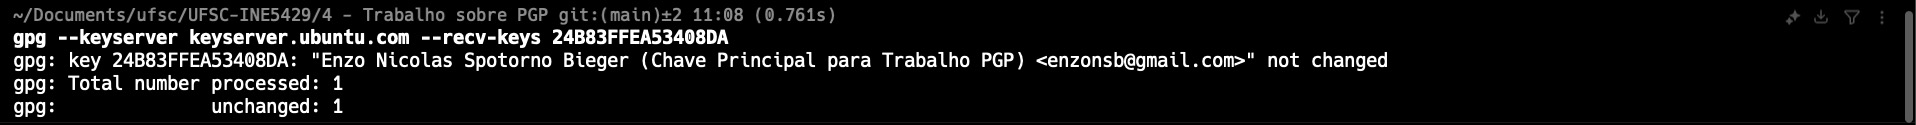
\includegraphics[width=0.8\textwidth]{images/03-importacao_chave_enzo_nicolas.jpg}
    \caption{Importação da chave do Enzo Nicolas}
    \label{fig:importacao-chave-enzo}
\end{figure}

\section{Verificação do Certificado}
Antes de assinar, foram verificadas as informações do certificado:

\begin{lstlisting}[language=bash]
# Listagem das chaves importadas para identificar a que se deseja assinar
gpg --list-keys

# Exibição de informações detalhadas sobre o certificado escolhido
gpg --fingerprint 4DE77B25F1F28B9F7A5BFB3E24B83FFEA53408DA
\end{lstlisting}

\begin{figure}[htb]
    \centering
    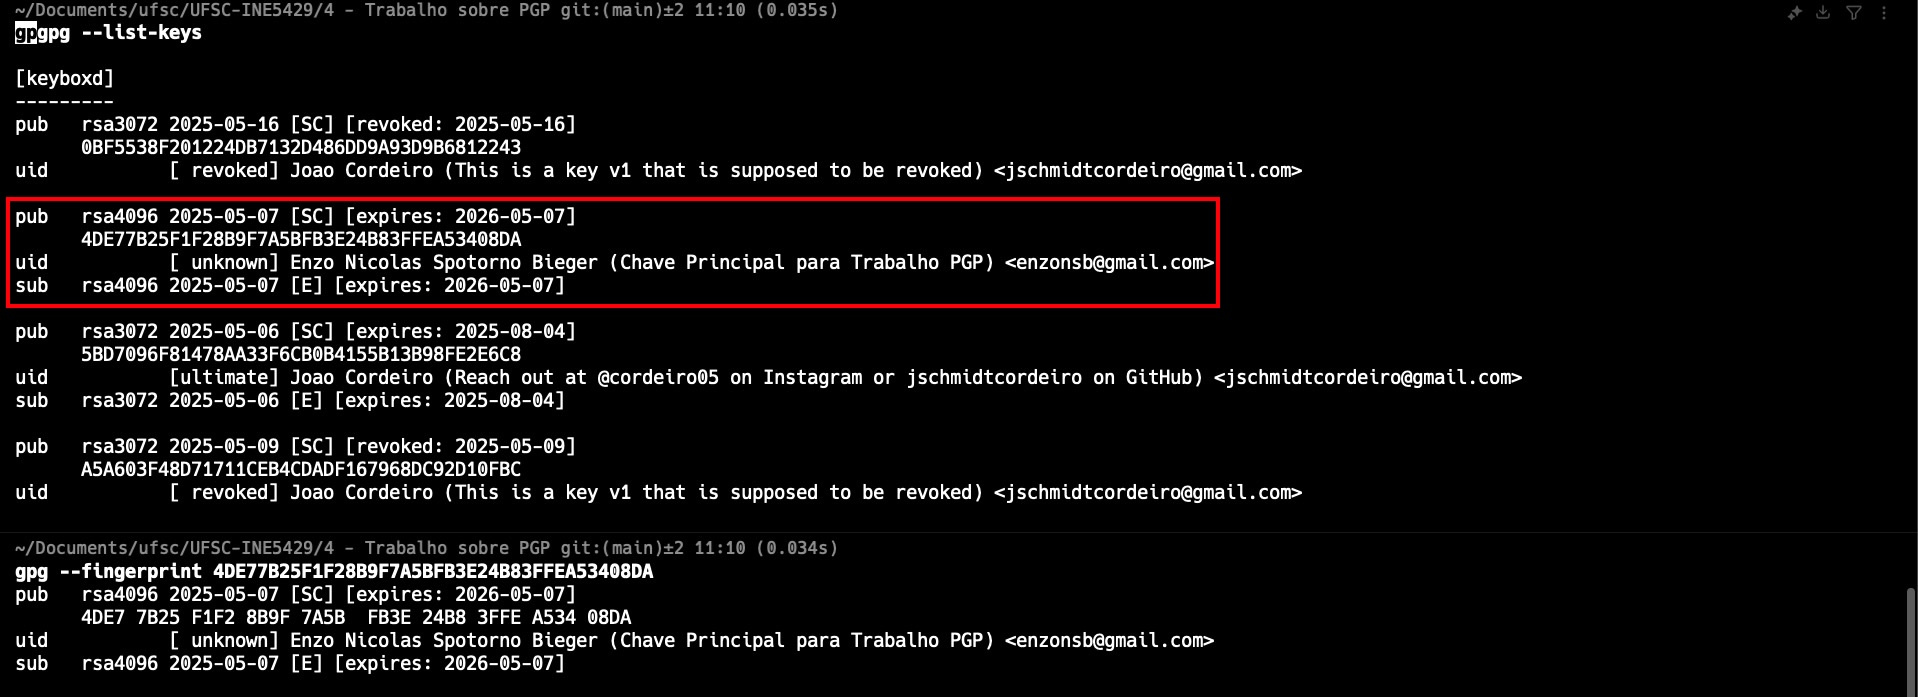
\includegraphics[width=0.8\textwidth]{images/03-verificacao_certificado.jpeg}
    \caption{Verificação do certificado}
    \label{fig:verificacao-certificado}
\end{figure}

\section{Assinatura do Certificado}
Após verificar a identidade do proprietário do certificado, procedeu-se com a assinatura \cite{gnupgkeysigning}:

\begin{lstlisting}[language=bash]
# Assinatura do certificado
gpg --sign-key 4DE77B25F1F28B9F7A5BFB3E24B83FFEA53408DA
\end{lstlisting}

\begin{figure}[htb]
    \centering
    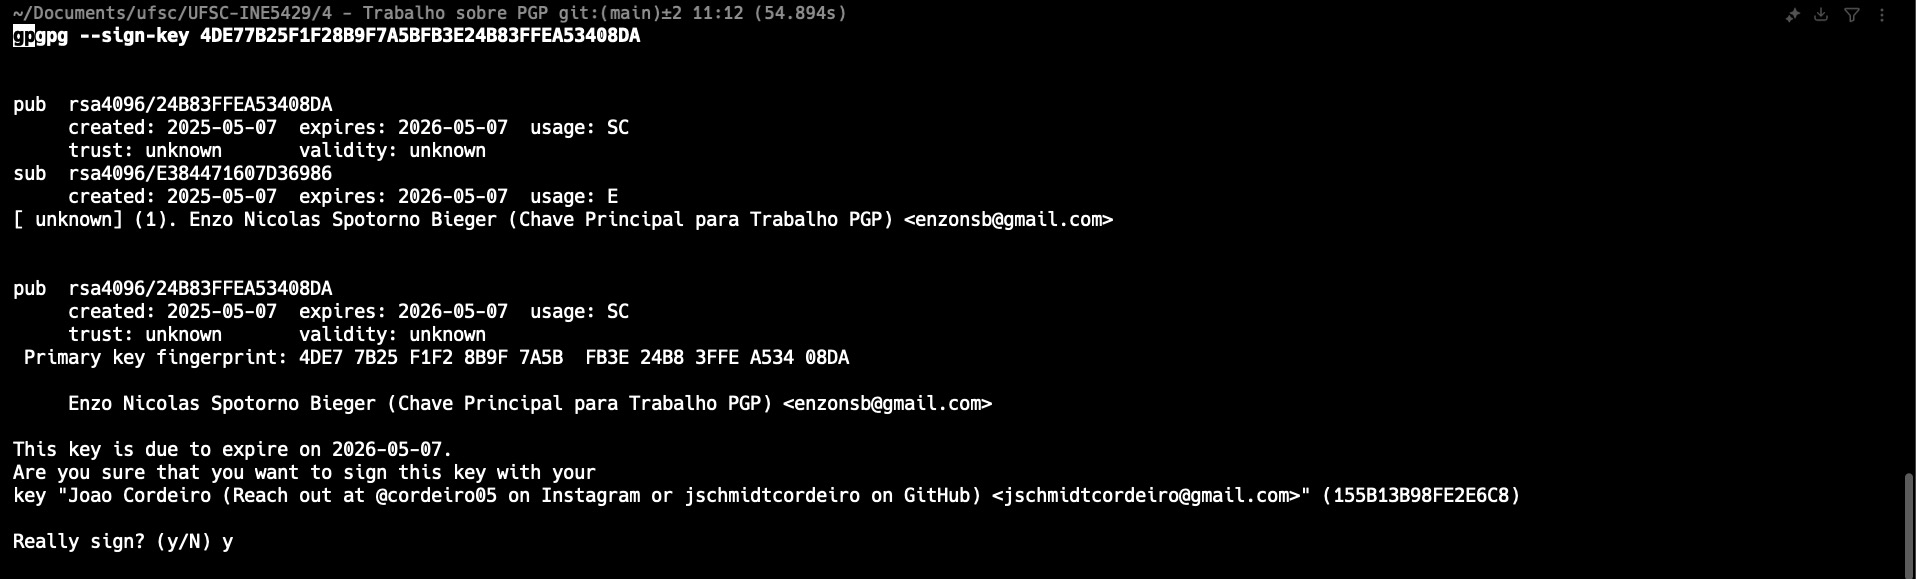
\includegraphics[width=0.8\textwidth]{images/03-assinatura_certificado.jpg}
    \caption{Assinatura do certificado}
    \label{fig:assinatura-certificado}
\end{figure}

Durante o processo interativo, foi confirmada a assinatura do certificado.

\section{Envio da Assinatura para o Servidor PGP}
Após assinar o certificado, a chave atualizada foi enviada para o servidor de chaves:

\begin{lstlisting}[language=bash]
# Envio do certificado assinado para o servidor
gpg --keyserver keyserver.ubuntu.com --send-key 4DE77B25F1F28B9F7A5BFB3E24B83FFEA53408DA
\end{lstlisting}

\begin{figure}[htb]
    \centering
    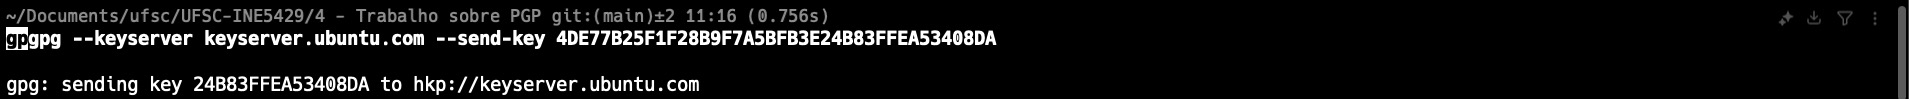
\includegraphics[width=0.8\textwidth]{images/03-envio_assinatura_servidor.jpg}
    \caption{Envio da assinatura para o servidor}
    \label{fig:envio-assinatura-servidor}
\end{figure}

\section{Verificação da Assinatura}
Para confirmar que a assinatura foi publicada com sucesso:

\begin{lstlisting}[language=bash]
# Atualização do chaveiro local com as informações do servidor
gpg --keyserver keyserver.ubuntu.com --refresh-keys

# Verificação do certificado para confirmar a assinatura
gpg --check-signatures 4DE77B25F1F28B9F7A5BFB3E24B83FFEA53408DA
\end{lstlisting}

\begin{figure}[htb]
    \centering
    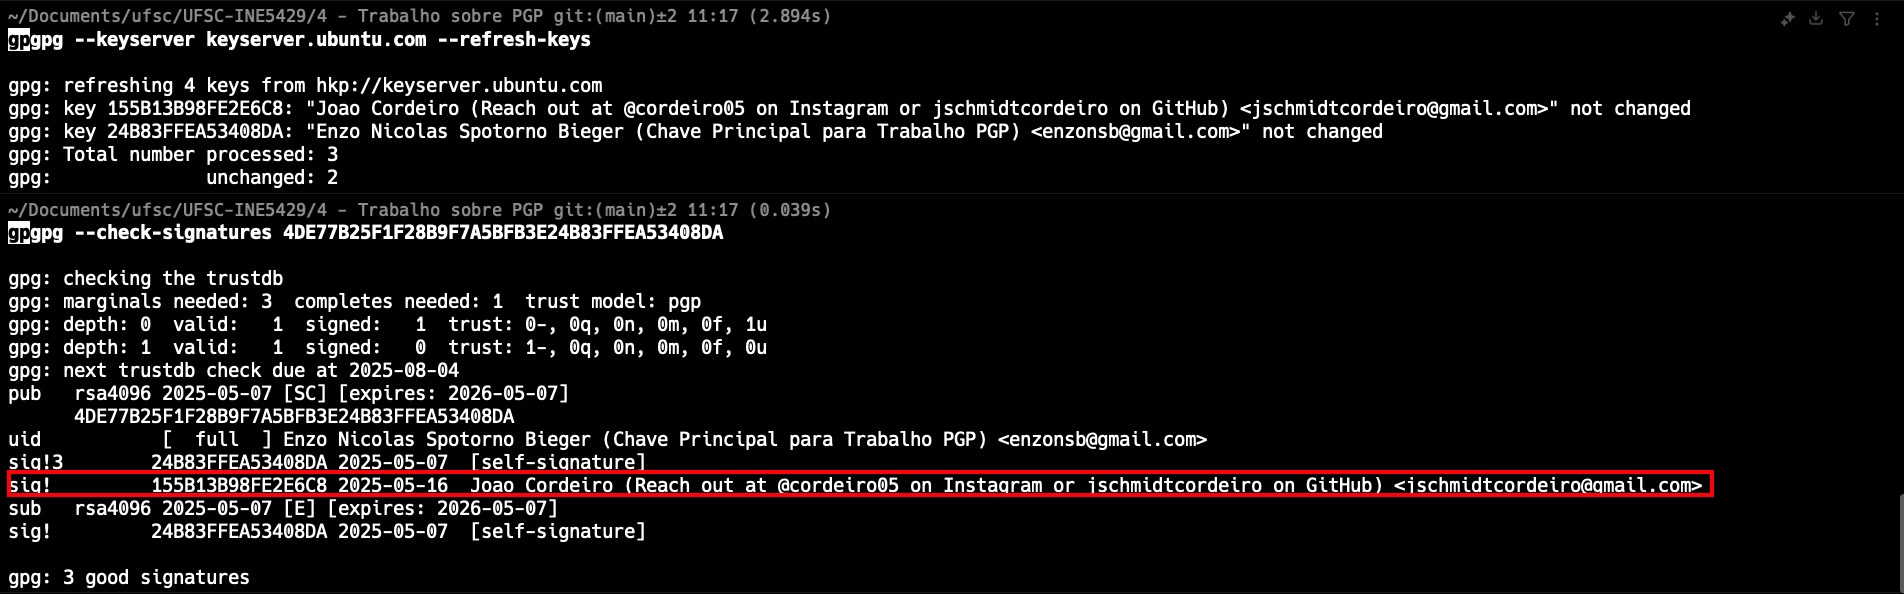
\includegraphics[width=0.8\textwidth]{images/03-verificacao_assinatura.jpeg}
    \caption{Verificação da assinatura}
    \label{fig:verificacao-assinatura}
\end{figure}

A saída mostra a assinatura associada ao certificado.

\section{Revogação da Assinatura}
Em seguida, procedeu-se com a revogação da assinatura \cite{rfc4880}:

\begin{lstlisting}[language=bash]
# Revogação da assinatura do certificado (processo interativo)
gpg --local-user 5BD7096F81478AA33F6CB0B4155B13B98FE2E6C8 --edit-key 4DE77B25F1F28B9F7A5BFB3E24B83FFEA53408DA
\end{lstlisting}

\begin{figure}[htb]
    \centering
    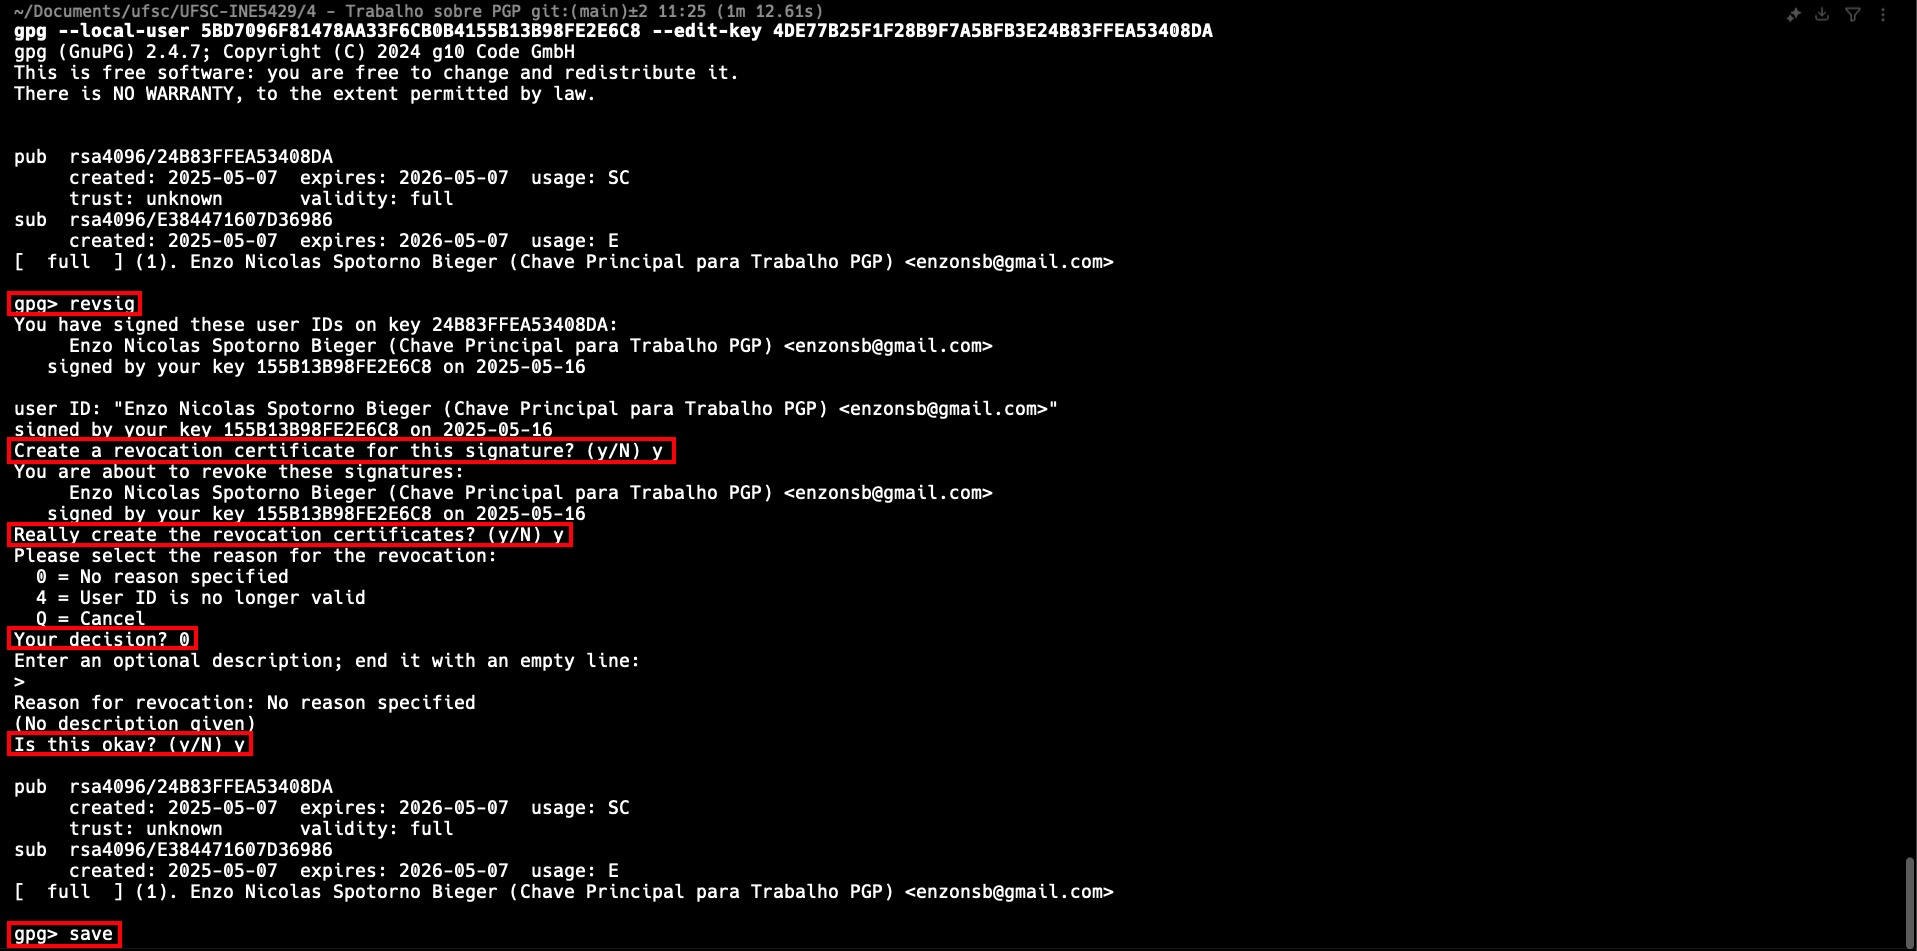
\includegraphics[width=0.8\textwidth]{images/03-revogacao_assinatura.jpeg}
    \caption{Revogação da assinatura}
    \label{fig:revogacao-assinatura}
\end{figure}

Durante o processo interativo:
\begin{enumerate}
    \item No prompt do GPG, foi digitado \texttt{revsig}
    \item Foi selecionado o ID de usuário correspondente (geralmente 1)
    \item A revogação foi confirmada quando solicitada
    \item Um motivo para a revogação foi escolhido (0-3)
    \item Uma descrição opcional foi fornecida
    \item O comando \texttt{save} foi utilizado para salvar as alterações e sair
\end{enumerate}

\section{Envio da Revogação para o Servidor}
Após revogar a assinatura, a chave atualizada foi enviada para o servidor:

\begin{lstlisting}[language=bash]
# Envio do certificado com a assinatura revogada para o servidor
gpg --keyserver keyserver.ubuntu.com --send-key 4DE77B25F1F28B9F7A5BFB3E24B83FFEA53408DA
\end{lstlisting}

\begin{figure}[htb]
    \centering
    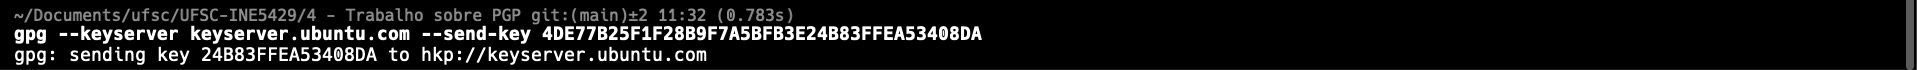
\includegraphics[width=0.8\textwidth]{images/03-envio_revogacao_servidor.jpg}
    \caption{Envio da revogação para o servidor}
    \label{fig:envio-revogacao-servidor}
\end{figure}

\section{Verificação da Revogação}
Para confirmar que a revogação da assinatura foi processada com sucesso:

\begin{lstlisting}[language=bash]
# Atualização do chaveiro local
gpg --keyserver keyserver.ubuntu.com --refresh-keys

# Verificação do certificado para confirmar a revogação da assinatura
gpg --check-signatures 4DE77B25F1F28B9F7A5BFB3E24B83FFEA53408DA
\end{lstlisting}

\begin{figure}[htb]
    \centering
    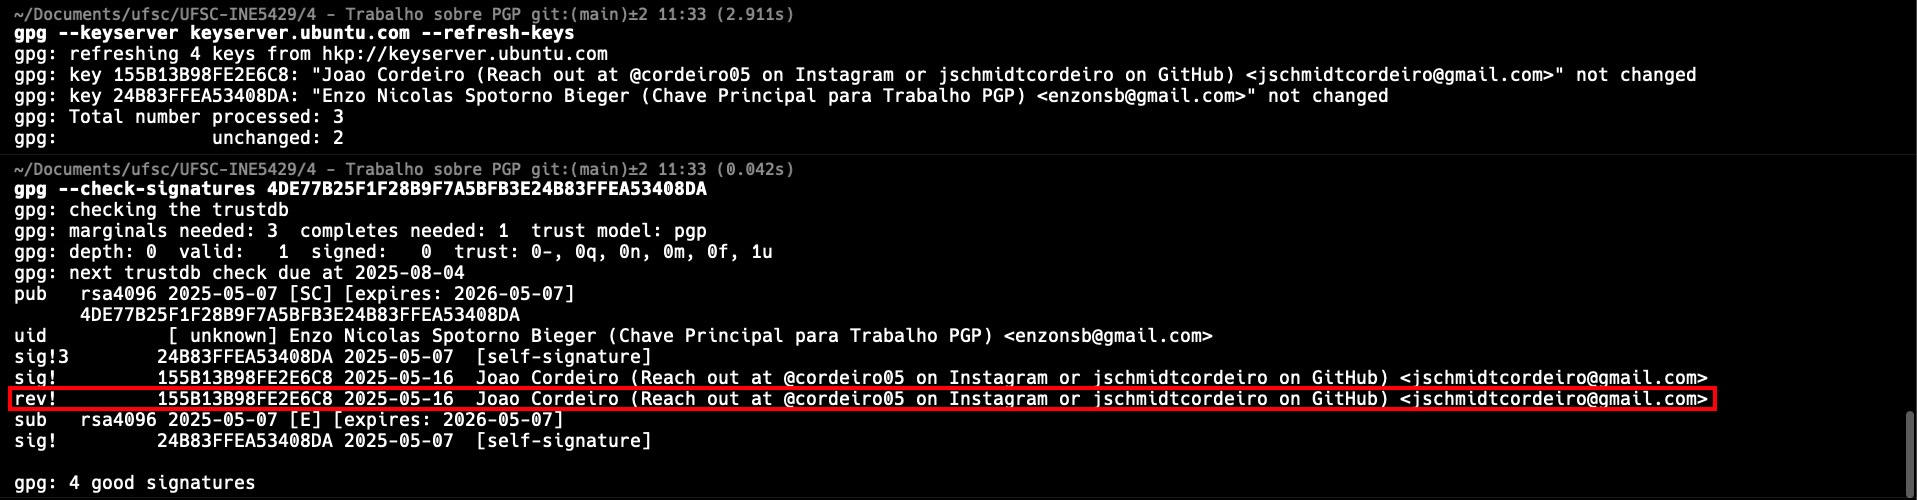
\includegraphics[width=0.8\textwidth]{images/03-verificacao_revogacao.jpeg}
    \caption{Verificação da revogação}
    \label{fig:verificacao-revogacao-assinatura}
\end{figure}

A saída mostra a assinatura como revogada.

\section{Resultados do Experimento}

Os resultados de cada comando dos experimentos estão disponíveis nas capturas de tela em suas respectivas seções. As informações principais sobre a assinatura revogada são:

\begin{itemize}
    \item \textbf{KeyID do certificado cuja assinatura foi revogada}: 4DE77B25F1F28B9F7A5BFB3E24B83FFEA53408DA
    \item \textbf{Data da assinatura}: 16 de maio de 2025
    \item \textbf{Data da revogação da assinatura}: 16 de maio de 2025
\end{itemize}